\subsubsection{VECMA toolkit}\label{sec:vecmatk}
%ref~\cite{Gr19Mast}
\begin{figure}
\centerline{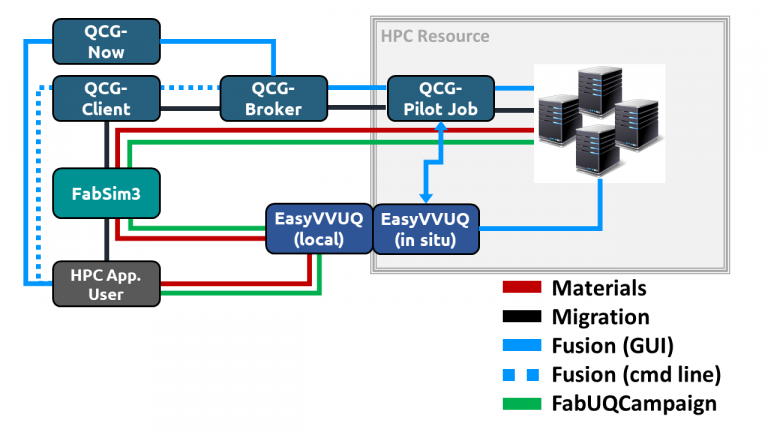
\includegraphics[width=0.9\textwidth]{../png/vecmatk}}
\caption{Usage of VECMAtk, taken from the website~\cite{vecmatkwebsite}. 
\label{fig:vecma}}
\end{figure}

%Co20When
The Verified Exascale Computing for Multiscale Applications~(VECMA) project~\cite{vecmawebsite}
in many important respects follows-on from the Computing Patterns for High
Performance Multiscale Computing~(ComPat) project~\cite{compatwebsite}.
Thus the ComPat website~\cite{compatswwebsite} lists the following software
\begin{itemize}
\item FabSim
\item QCG -- Quality in Cloud and Grid
\item MUSCLE 2 -- The Multiscale Coupling Library and Environment
\end{itemize}

whereas the VECMA toolkit~(VECMAtk) website~\cite{vecmatkwebsite} lists 
(and provides links to):
\begin{itemize}
\item FabSim3
\item QCG Pilot Job~(QCGPJ), QCG-Now, QCG-Broker  and QCG-Client
\item MUSCLE 3
\item EasyVVUQ --  Facilitate verification, validation and uncertainty quantification (VVUQ) 
\item EasyVVUQ-QCGPJ
\end{itemize}
where the EasyVVUQ software represents the VVUQ capability developed by the
VECMA project.

The roles played by FabSim, QCG and MUSCLE~2 appear to have been taken over by
FabSim3, QCGPJ and MUSCLE~3 respectively in the more recent project, and as
they are described in \Sec{compat} will not be described further. 

MUSCLE~3, updating MUSCLE~2, is effectively a separate development from VECMAtk, that provides a coupling
capability between different codes. It is of additional interest because it has
the capability not only to implement but also to create couplings using the 
Multiscale Modeling and Simulation Language~(MMSL) which was developed in tandem
with the original MUSCLE. Unfortunately, as of mid-2020, there is no further 
funding for developing or supporting MUSCLE~3, but it will continue to be 
supported by Lourens Veen at the Netherlands eScience center in his ``spare~time".

\Fig{vecma} indicates how the components of VECMAtk, apart from MUSCLE~3
(which would be confined to the HPC Resource), interact.
VECMA toolkit is not a software pattern in the strict sense in that
it typically spans a network. The QCG software devloped in Poland at
the Poznan Supercomputing and Networking Center~(PSNC) provides the
user with a system-independent
approach to the problem of executing a set of interrelated jobs on
a cluster of machines or as indicated in the figure, a HPC machine in the
background. QCG-Now is a desktop GUI interface to the other components
of the QCG-Client, of which the most important for VECMAtk is QCGPJ.
EasyVVUQ~\cite{Ri20Easy} is a Python library to help produce computational ``campaigns"
to enable UQ of simulations on HPC machines in combination with QCGPJ,
with which it is specially packaged as EasyVVUQ-QCGPJ. The intent appears to be that
EasyVVUQ-QCGPJ will replace FabSim3 which provides similar functionality also using Python.

The basic pattern in EasyVVUQ-QCGPJ is in fact the straightforward~\cite{Wr20Buil}
\begin{enumerate}
\item Produce ensemble of calculations (``campaign"),
\item Execute unmodified simulation code for each set of parameters
\item Correlate results of ensemble
\end{enumerate}
so that EasyVVUQ-QCGPJ is non-intrusive in the sense that like most UQ packages
it simply wrappers existing code.  Indeed it exploits Feinberg's chaospy library~\cite{Fe15chao}
to help generate the ensembles via sampling from distributions provided by the 
library~\cite{chaospywebsite}.

%One point to note regarding the VECMA project is the use of the term semi-intrusive
%in the context of a multiscale workflow, to mean typically that the outputs from an
%ensemble of small-scale calculations are not only combined but also further processed,
%eg. used to fit a simple parametric model, which feeds into the larger scale rather
%than say the ensemble average. This conflicts with the use of the term by
%Abgrall~et~al~\cite{Ab13semi} to describe a minimally intrusive technique, where
%in the example given, iterates are averaged over a distribution as solution
%proceeds.

